Although the Freebase knowledge graph is not maintained anymore since it was integrated into Wikidata~\cite{Tanon2016FromFT}, the benchmark datasets derived from it are still widely used. One popular~\cite{Toutanova2015RepresentingTF} benchmark dataset is the \emph{FB15k} dataset introduced by Bordes et al. in 2013~\cite{Bordes2013TranslatingEF} whose name resembles the fact that it covers roughly \num{15000} Freebase entities. On its basis, Toutanova and Chen introduced the FB15k-237~\cite{Toutanova2015ObservedVL} in 2015 whose purpose was to create a more meaningful benchmark by eliminating trivially predictable facts. For example, if FB15k-237 covers a relation like $(x, contains, y)$, it does not include its inverse relation $(y, part~of, x)$, because good performance resulting from such trivial, mutual predictions detracts from more interesting cases. In 2020, Safavi and Koutra were pushing this further and published the CoDEx datasets, which are derived from FB15k-237 and two other datasets, that cover more diverse content and are again more difficult than FB15k~\cite{Safavi2020CoDExAC}. From the three provided datasets CoDEx-S, CoDEx-M and CoDEx-L, the IRT split by Hamann, on which this work is based, focuses on the CoDEx-M dataset. Table~\ref{tab:5_experiments/1_base_datasets/1_knowledge_graphs/benchmark_datasets} gives an overview of FB15k, FB15k-237 and CoDEx-M.

\begin{table}[h]
    \centering
    \begin{tabular}{| l | r | r | r | r | r |}
    \hline

    \multicolumn{1}{|c|}{\textbf{Dataset}} &
    \multicolumn{1}{|c|}{\textbf{#Entities}} &
    \multicolumn{1}{|c|}{\textbf{#Relations}} &
    \multicolumn{3}{|c|}{\textbf{#Facts}} \\

    \multicolumn{1}{|c|}{} &
    \multicolumn{1}{|c|}{} &
    \multicolumn{1}{|c|}{} &
    \multicolumn{1}{|c|}{\textbf{Train}} &
    \multicolumn{1}{|c|}{\textbf{Valid}} &
    \multicolumn{1}{|c|}{\textbf{Test}} \\

    \hline \hline

    FB15k     & \num{14951} & \num{1345} & \num{483142} & \num{50000} & \num{59071} \\
    FB15k-237 & \num{14541} & \num{237}  & \num{272115} & \num{17535} & \num{20466} \\
    CoDEx-M   & \num{17050} & \num{51}   & \num{185584} & \num{10310} & \num{10311} \\

    \hline
\end{tabular}

    \caption{Popular KGC benchmark datasets}
    \label{tab:5_experiments/1_base_datasets/1_knowledge_graphs/benchmark_datasets}
\end{table}

As for the above KGC benchmark datasets, a graph's fact subset is usually further split into training, validation and test subsets, although it should be mentioned that the CoDEx-M split actually provides additional sets of certainly non-true facts not listed in table~\ref{tab:5_experiments/1_base_datasets/1_knowledge_graphs/benchmark_datasets}. Thereby, the splits are created so that there are training, validation and test facts for possibly every entity. In contrast, in his work on zero-shot prediction, Hamann creates new splits from FB15k-237 and CoDEx-M that distinguish between so-called \emph{closed-world (CW) entities}, seen during training, and \emph{open-world (OW) entities}, that are not seen during training, to optimize prediction for unknown entities.

\begin{figure}
    \centering
    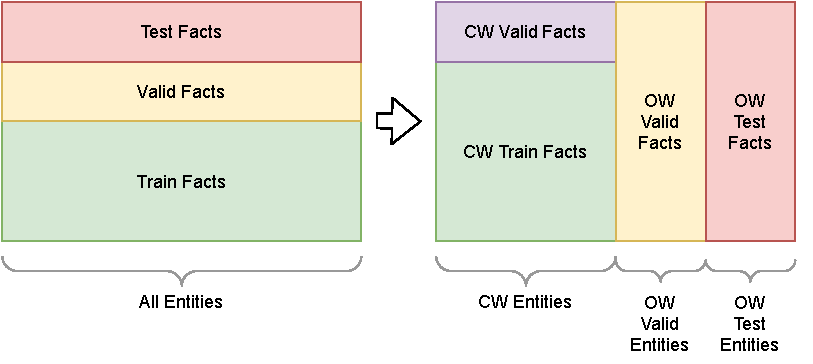
\includegraphics[width=\textwidth]{5_experiments/1_base_datasets/1_knowledge_graphs/irt_split}
    \caption{Comparison of (a) conventional and (b) the IRT fact split for KGC}
    \label{fig:5_experiments/1_base_datasets/1_knowledge_graphs/irt_split}
\end{figure}

Figure~\ref{fig:5_experiments/1_base_datasets/1_knowledge_graphs/irt_split} illustrates the difference between the approaches. The closed-world entities' facts are further split into closed-world training and closed-world validation facts to support closed-world prediction in addition to open-world prediction. Closed-world training and closed-world validation facts only refer to closed-world entities, while at least one of an open-world facts' head or tail refers to an open-world entity. The open-world entities properly divided into disjoint subsets of open-world validation and open-world test entities that do not appear in each other's fact sets. Table~\ref{tab:5_experiments/1_base_datasets/1_knowledge_graphs/irt_splits} gives an overview of the entity and fact sets' dimensions. For readability, the rest of the chapter will occasionally refer to IRT's FB15k-237 and CoDEx-M splits as FB and CDE, respectively. Also, "training", "validation" and "entities" will be often abbreviated to "train", "valid" and "ents" in figures and tables.

\begin{table}[h]
    \centering
    \begin{tabular}{ l c r r r c r r c r r }
    \toprule
    
    \multicolumn{1}{l}{\textbf{Graph}} & \phantom &
    \multicolumn{1}{c}{\textbf{\thead{CW \\ Train \\ Ents}}} &
    \multicolumn{1}{c}{\textbf{\thead{CW \\ Train \\ Facts}}} &
    \multicolumn{1}{c}{\textbf{\thead{CW \\ Valid \\ Facts}}} & \phantom &
    \multicolumn{1}{c}{\textbf{\thead{OW \\ Valid \\ Ents}}} &
    \multicolumn{1}{c}{\textbf{\thead{OW \\ Valid \\ Facts}}} & \phantom &
    \multicolumn{1}{c}{\textbf{\thead{OW \\ Test \\ Ents}}} &
    \multicolumn{1}{c}{\textbf{\thead{OW \\ Test \\ Facts}}} \\

    \midrule

    FB15k-237 && \num{12057} & \num{214412} & \num{23778} && \num{1545} & \num{46503} && \num{816}  & \num{25423} \\
    CoDEx-M   && \num{11399} & \num{123650} & \num{13738} && \num{2918} & \num{41240} && \num{1896} & \num{27577} \\

    \bottomrule
\end{tabular}

    \caption{IRT Split Sizes}
    \label{tab:5_experiments/1_base_datasets/1_knowledge_graphs/irt_splits}
\end{table}
